% !TeX root = main.tex
\chapter{Architectural Foundations of DNN Acceleration}
\label{ch:foundations}

% Chapter Introduction
The efficient execution of Deep Neural Networks (DNNs) presents one of the most significant challenges and opportunities in modern computer architecture. While today's general-purpose CPUs are highly optimized for a wide range of tasks, their fundamental design principles are often mismatched with the unique computational and data movement patterns of large-scale neural networks. This chapter will establish the foundational concepts that motivate the need for specialized hardware. We will begin by exploring the core problem---the immense cost of data movement---and then introduce the classic architectural paradigm designed to solve it: the systolic array. Finally, we will examine how this timeless principle is embodied in state-of-the-art industrial accelerators, providing the necessary context to understand the design of the Gemmini accelerator, which is the central subject of this thesis.

\section{The Data-Compute Divide: The Memory Wall}
\label{sec:memory_wall}

The performance of any computing system is ultimately limited by two factors: the speed of its computations and the speed at which it can supply data to its computational units. For decades, Moore's Law drove exponential growth in the number of transistors on a chip, leading to dramatic increases in processing power. However, the speed of off-chip memory systems, such as DRAM, has improved at a much slower pace. This growing disparity between processor speed and memory speed is famously known as the \textbf{Memory Wall} \cite{wulf1995hitting}.

For data-intensive workloads like DNNs, this is the primary performance bottleneck. The problem can be understood with a simple analogy: imagine a master chef (the processor) who can perform culinary tasks with superhuman speed. However, their ingredients (the data) are stored in a large warehouse across the street (DRAM). Even though the chef is exceptionally fast, their overall productivity is dominated by the time spent walking to and from the warehouse to fetch each ingredient.

This bottleneck is not just about latency; it is fundamentally about energy. As quantified by Horowitz \cite{horowitz2014energy}, the energy required to perform a complex 32-bit floating-point computation is dwarfed by the energy needed to fetch its operands from off-chip DRAM (Figure \ref{fig:energy_cost}). This immense energy cost of data movement means that for DNNs, which perform billions of operations, any viable high-performance hardware solution must be designed with a primary objective: to minimize data movement.

\begin{figure}[h!]
    \centering
    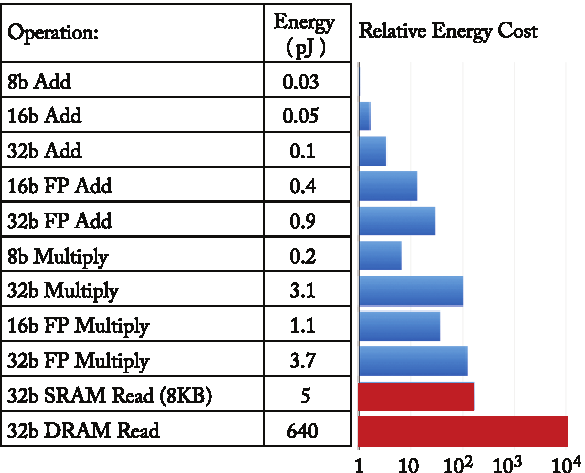
\includegraphics[width=0.8\textwidth]{EfficientDNN_EnergyConsumption.pdf} 
    \caption[The Relative Energy Cost of Computation vs. Memory Access]{The relative energy cost of various arithmetic and memory operations. A 32-bit DRAM read is orders of magnitude more costly than a 32-bit floating-point addition. This disparity is the primary motivation for specialized accelerator architectures. Adapted from Horowitz, as presented in Sze et al. \cite{sze2020efficient, horowitz2014energy}.}
    \label{fig:energy_cost}
\end{figure}

\section{A Classic Solution: The Systolic Principle}
\label{sec:systolic_principle}

In his seminal 1982 paper, H.T. Kung proposed a novel architectural paradigm designed specifically to address the memory wall: the \textbf{systolic array} \cite{kung1982systolic}. The architecture is named by analogy to the human circulatory system. Just as the heart rhythmically pumps blood to the body's cells, in a systolic system, memory "pumps" data through a regular grid of simple Processing Elements (PEs).

The core principle is to \textbf{maximize the number of computations performed for each data item fetched from memory}. Instead of fetching an operand, using it once in a central ALU, and then discarding it (the conventional approach), a systolic array passes an operand from one PE to the next in a pipelined fashion. At each step of its journey, the data element participates in another computation. This structure, illustrated conceptually in Figure \ref{fig:conventional_vs_systolic}, amortizes the high cost of the initial memory access over dozens or even hundreds of useful operations.

\begin{figure}[htbp]
    \centering
    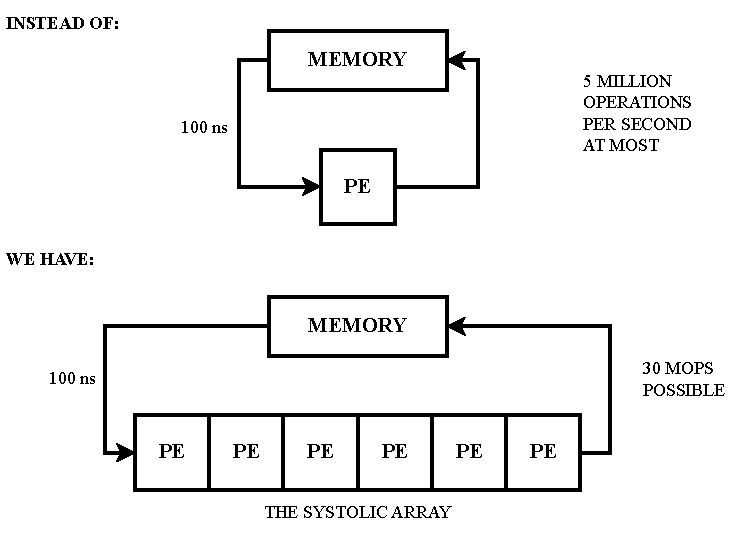
\includegraphics[width=0.9\textwidth]{SystolicArray_Kung1982.pdf} 
    \caption[Conventional vs. Systolic Processing]{A conceptual comparison of a conventional von Neumann architecture and a systolic architecture. The conventional approach (top) is bottlenecked by the memory bus. The systolic approach (bottom) uses an array of PEs to achieve high throughput with the same memory bandwidth by reusing data internally. Adapted from the presentation of Kung's work \cite{kung1982systolic}.}
    \label{fig:conventional_vs_systolic}
\end{figure}

\section{Case Studies in Modern Systolic Design}
\label{sec:case_studies}
While the systolic principle is four decades old, it has become the dominant paradigm for modern high-performance DNN accelerators. We will examine two landmark industrial designs that showcase this principle in practice.

\subsection{Google's TPUv1: A Datacenter-Scale Design}
Google's Tensor Processing Unit (TPU) was one of the first large-scale custom ASICs designed specifically for accelerating DNN inference in datacenters \cite{jouppi2017tpu}. As shown in Figure \ref{fig:tpu_diagram}, its architecture is a direct embodiment of the systolic principle. The heart of the TPU is a massive 256x256 Matrix Multiply Unit, which is a two-dimensional systolic array of 65,536 8-bit multiply-accumulate (MAC) units. To feed this vast computational engine, the TPU relies on a large, software-controlled on-chip memory called the Unified Buffer (a 24 MiB scratchpad), which stores input activations and intermediate partial sums. The design philosophy of the TPU prioritizes deterministic, high-throughput performance for inference tasks where low latency is critical.

\begin{figure}[htbp]
    \centering
    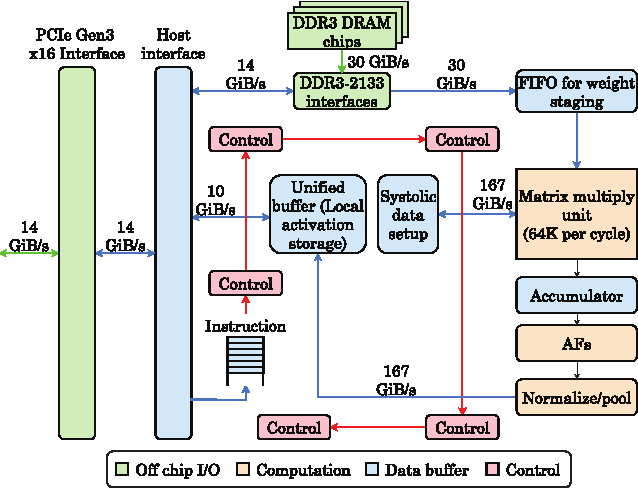
\includegraphics[width=\textwidth]{TPU_v1_Overview.pdf} 
    \caption[The Google TPUv1 Block Diagram]{A high-level block diagram of the Google TPUv1. The design is dominated by the systolic Matrix Multiply Unit and its large on-chip Unified Buffer. Adapted from Jouppi et al. \cite{jouppi2017tpu, mittal2021survey}.}
    \label{fig:tpu_diagram}
\end{figure}

\subsection{NVIDIA NVDLA: An Open-Source Accelerator IP}
In contrast to the monolithic, datacenter-focused TPU, the NVIDIA Deep Learning Accelerator (NVDLA) is an open-source, configurable IP core designed for integration into a wide range of Systems-on-Chip (SoCs), particularly for embedded systems \cite{farshchi2019nvdla}. As shown in Figure \ref{fig:nvdla_diagram}, the NVDLA has a more modular design, with a dedicated Convolutional Core (which contains the MAC units), a Post-Processing unit for activation functions and pooling, and a Convolutional Buffer for storing weights and inputs. Unlike the TPU's custom interface, the NVDLA uses industry-standard bus protocols (AXI and APB) for memory access and control, simplifying its integration into third-party SoC designs. Its configurability (e.g., `nv\_small`, `nv\_large`) allows a system designer to trade off area and performance, making it a flexible solution for the embedded space.

\begin{figure}[htbp]
    \centering
    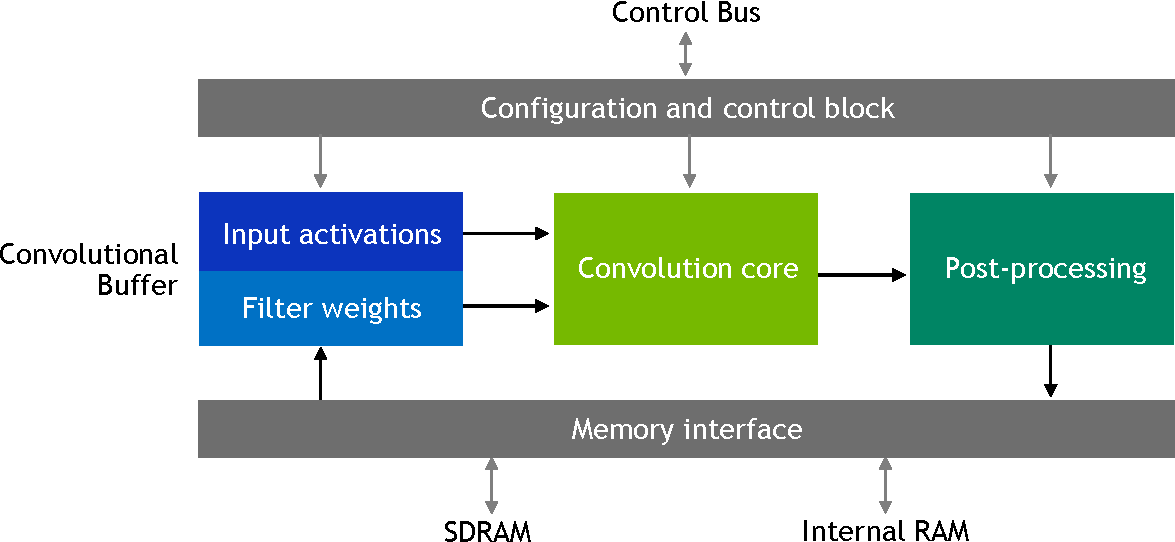
\includegraphics[width=\textwidth]{NVDLA_ArchitectureOverview.pdf} 
    \caption[The NVDLA High-Level Architecture]{The high-level architecture of the NVDLA. The design is partitioned into distinct functional units connected via standard bus interfaces. Adapted from Farshchi et al. \cite{farshchi2019nvdla}.}
    \label{fig:nvdla_diagram}
\end{figure}

\section{A Formal Framework: Dataflows}
\label{sec:formal_dataflows}
The design choices made in architectures like the TPU and NVDLA can be formally described using the concept of a \textbf{dataflow}. The dataflow defines the strategy for moving data through the systolic array to maximize reuse. The effectiveness of a given dataflow depends on the structure of the DNN layer being executed. The two most common dataflows, which we will see are directly relevant to Gemmini, are:
\begin{itemize}
    \item \textbf{Weight Stationary (WS):} This dataflow prioritizes weight reuse. Filter weights are pre-loaded into the PEs and remain stationary, while input activations are streamed in. This strategy, used by the Google TPU, is highly efficient for layers with large input feature maps and relatively small filters.
    \item \textbf{Output Stationary (OS):} This dataflow prioritizes minimizing the movement of partial sums. Each PE is responsible for accumulating the final value for a single output activation, which remains stationary in its accumulator. Inputs and weights are streamed to the PE as needed. This can be more efficient for layers where partial sum read/write energy is a dominant cost.
\end{itemize}
These strategies, visually contrasted in Figure \ref{fig:dataflow_taxonomy} and \ref{fig:dataflow_comparison}, represent a fundamental trade-off in accelerator design. The choice of dataflow directly impacts which types of data reuse, shown in Figure \ref{fig:dnn_reuse}, are most effectively exploited.

\begin{figure}[htbp]
    \centering
    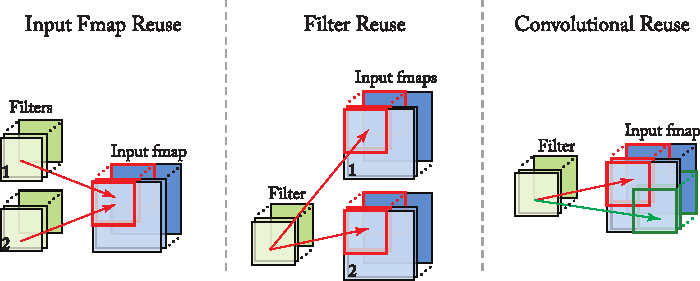
\includegraphics[width=0.9\textwidth]{EfficientDNN_DataReuse.pdf} 
    \caption[Data Reuse Opportunities in DNNs]{The three primary forms of data reuse in convolutional layers: convolutional, filter, and input reuse. Adapted from Sze et al. \cite{sze2020efficient}.}
    \label{fig:dnn_reuse}
\end{figure}

\begin{figure}[htbp]
    \centering
    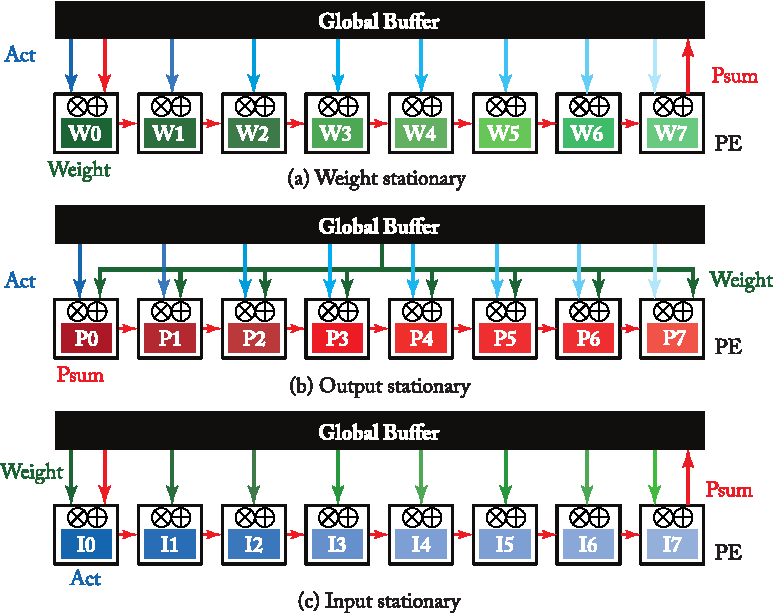
\includegraphics[width=0.9\textwidth]{EfficientDNN_ModernDataflow.pdf} 
    \caption[Taxonomy of Common DNN Dataflows]{A visual comparison of Weight Stationary (left) and Output Stationary (right) dataflows. Adapted from Sze et al. \cite{sze2020efficient}.}
    \label{fig:dataflow_taxonomy}
\end{figure}

\begin{figure}[htbp]
    \centering
    \begin{subfigure}[b]{0.48\textwidth}
        \centering
        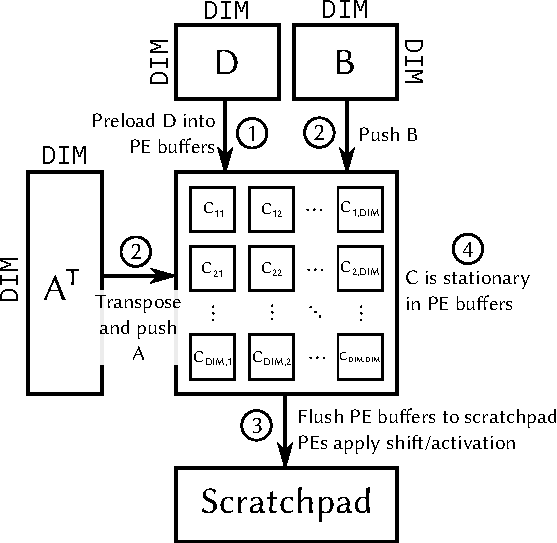
\includegraphics[width=\textwidth]{Gemmini_compute_os.pdf}
        \caption{Output Stationary (OS)}
        \label{fig:os_dataflow}
    \end{subfigure}
    \hfill
    \begin{subfigure}[b]{0.48\textwidth}
        \centering
        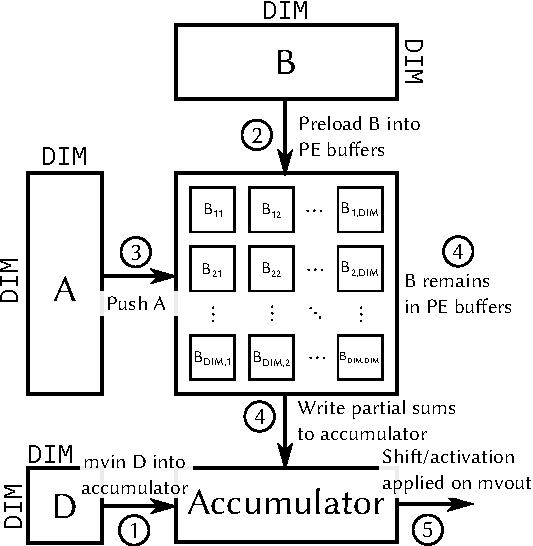
\includegraphics[width=\textwidth]{Gemmini_compute_ws.pdf}
        \caption{Weight Stationary (WS)}
        \label{fig:ws_dataflow}
    \end{subfigure}
    \caption[Comparison of OS and WS Dataflows]{A visual comparison of the two primary dataflows supported by Gemmini. (a) In the \textbf{Output Stationary} dataflow, the result matrix C remains stationary in the PEs to accumulate partial sums. (b) In the \textbf{Weight Stationary} dataflow, the weight matrix B is preloaded and remains stationary in the PEs to maximize weight reuse. The choice between these strategies represents a fundamental trade-off in accelerator design. Source: \cite{gemini-dac}.}
    \label{fig:dataflow_comparison}
\end{figure}

\section{Chapter Summary}
This chapter has built a foundational argument for the necessity of specialized hardware for DNN acceleration. We began with the core architectural challenge---the Memory Wall---and introduced the systolic array as a classic and enduring solution that minimizes costly data movement by maximizing data reuse. By examining modern industrial accelerators like the Google TPU and NVDLA, we have seen this principle in action. Finally, we formalized these strategies with the concept of dataflows, such as Weight Stationary and Output Stationary. These foundational concepts provide the necessary framework to understand the design and operation of the Gemmini accelerator, which will be the focus of the subsequent chapters.